\documentclass[a4paper]{article}

\usepackage[utf8]{inputenc}

\usepackage{url}
\usepackage[hidelinks]{hyperref}

\usepackage{caption}

\usepackage{listings}

\usepackage{color}

% *** GRAPHICS RELATED PACKAGES ***
%\usepackage[pdftex]{graphicx}
\usepackage{graphicx}
%\usepackage[dvips]{graphicx}
% to place figures on a fixed position
\usepackage{float}

\usepackage[margin=1in]{geometry}

\title{P2P – syllabus}
\author{}
\date{}


\begin{document}

\maketitle

\tableofcontents

\section{Introduction}

Compared to traditional client-server connections peer-to-peer solutions (P2P) offer more direct and dynamic alternatives. They provide searching services in a global network and allow direct, point to point data transfers bypassing the administrative and performance bottlenecks of servers.
The well-know and most used P2P applications -- like file exchange, VoIP and on-line gaming -- affects many users and generate the significant portion of today's Internet traffic. Covering all aspects of P2P network during this lab would be impossible therefore only some key parts will be demonstrated. Since file transfer is currently to most utilized application we are going to cover that during this lab.

\section{P2P file exchange}

Az első speciálisan fájlok egymás közötti cseréjére kifejlesztett rendszer, a Napster 1999-ben jelent meg. A fájlcserélő hálózatok utána igen gyorsan fejlődtek, rengeteg architektúra alakult ki, melyeket három fő kategóriába sorolhatunk. A fejezet bemutatja az egyes kategóriákat, majd pedig részletesen a BitTorrentet, amellyel a mérés során megismerkedünk.

\subsubsection{Client-server systems}

A Napster hálózat felépítése igen egyszerű. A rendszer alapját egyetlen szerverközpont alkotja. Minden egyes felhasználó ehhez a szerverhez kapcsolódik kliensprogramjával. Az állományok letöltése is a szerver vezérlésével történik, azonban maga az állomány áttöltés már közvetlenül a kérő és kínáló kliens között történik, a szerver érintése nélkül. E tulajdonsága miatt nevezhetjük a Napstert peer-to-peer hálózatnak, hiszen kiaknázza a hálózat minden egyes felhasználójánál rejlő tárolókapacitást, illetve sávszélességet. A Napster hálózat nyilvánvaló hátránya, hogy egyetlen központi szerverre (szerverparkra) hagyatkozik, melynek esetleges bezárása az egész hálózat leállításával jár. Erre számos esetben sor is került, mert a RIAA (amerikai jogvédő szerv) sorozatosan perelte a Napstert az illegálisan megosztott tartalmak miatt.

Egyesek ezért az architektúra alapjait próbálták módosítani, és olyan megoldást kerestek, amely nem támaszkodik központi elemekre, ehelyett teljesen elosztott. Mások viszont csak a biztonsági problémák leküzdésére koncentráltak, és csak az ehhez szükséges módosításokat akarták végrehajtani az architektúrán. Így egy olyan rendszerhez jutottak, melyben ugyan egy központi entitáshoz csatlakoznak a kliensek, azonban egyrészt semmilyen információt nem tárol a kliensekről, másrészt pedig nem egyetlen szervert üzemeltettek, hanem ehelyett számos kisebb szervert nyitottak meg. A legjelentősebb ilyen architektúra a DirectConnect.

\subsubsection{Distributed systems}

A Napster bukása után rájöttek, hogy az állománymegosztó rendszereknél az egyik fő sebezhetőséget a központi szerver jelenléte okozza. Később a DirectConnect alapú hálózatok sorozatos támadása miatt a legtöbb állománycserélő felhasználó olyan rendszerarchitektúrát kezdett keresni, amely teljesen elosztott, vagyis egyáltalán nem tartalmaz központi entitást. Az elosztott architektúra ugyanakkor számos hátrányt jelent a korábbi kliens-szerver jellegi működéshez képest. Itt ugyanis az egyes kliensek az architektúrában nemcsak kétugrásnyi távolságra vannak egymástól, hanem tetszőlegesen nagy távolságra is lehetnek. Emiatt egy kérés jelentősen nagyobb forgalmat generál a hálózat egészében, valamint sokkal nagyobb időt vesz igénybe annak végrehajtása és a válaszok megszerzése. További elvi problémát jelent, hogy mostantól nem triviális a hálózatba való beléptetés, hiszen nincs központi elem, így egy új felhasználó kénytelen valamely hálózati tag címét megismerni, ugyanakkor az adminisztráció is szinte lehetetlenné válik.

A 2000-es korszakot rengeteg ilyen elven alapuló hálózat jellemzi. Ebben az időben szinte minden programozó szabadidejében peer-to-peer állománymegosztó programokat fejlesztett. Rengeteg különböző ötlet, megoldás született, ám ezek legtöbbje nem volt túl hosszú életű. Néhány rendszernek azonban sikerült fennmaradnia és nagy népszerűségre szert tennie, ilyen pl. a Gnutella, mely bizonyos országokban még ma is a legnépszerűbb hálózat.

A Gnutella hálózat teljesen peer-to-peer, vagyis csak az egymással kommunikáló kliensekből áll; nem használ semmilyen központi, vagy globálisan elérhető rendszerelemet. Ez máris egy új problémát vet fel, amellyel a korábbi rendszereknél nem találkozhattunk. A problémát az okozza, hogy mivel nincs központi elem, egy új kliensnek valamely, már a rendszer részét képező klienshez kell csatlakoznia, amihez elengedhetetlen, hogy legalább egyet ismerjen közülük. Erre eredetileg nem volt kész megoldás, így tulajdonképpen szájról szájra járt egy-egy kliens címe, amihez a felhasználók csatlakoztak. Megjelentek még különböző keresési algoritmusok is, ám ezek nem működtek túl hatékonyan globális méretekben.

Miután a kliens megismert egy Gnutella tagot, kezdeményezi a csatlakozást hozzá. Ehhez egy üdvözlő üzenetet használ. A peer, aki megkapja ezt az üzenetet, válaszol rá, tudatva, hogy még mindig aktív. Ezen kívül továbbítja a csomagot minden más peernek, akit ismer a hálózatban – természetesen csökkentve az üdvözlő üzenet életben maradási idejét. Ez a folyamat ismétlődik, míg nullára nem csökken az üdvözlés életben maradási ideje. Eközben az üzenet igen sok tagot látogatott meg, tulajdonképpen a csatlakozásra kiválasztott peertől számított hatos mélységben minden egyes tagot. Ezekkel mind felveszi a kapcsolatot az új becsatlakozó, így a csatlakozási procedúra lezajlása után szorosan kapcsolódik a rendszerhez.

A jogi támadhatóság ellen is szinte teljes biztonságot kínál, hiszen a hálózat szinte feltérképezhetetlen. A feltérképezhetetlenség egyébként egyben az architektúra egyik nagy hátránya is, hiszen a kliensek kis horizontja miatt az Internet teljes monitorozása nélkül lehetetlen képet alkotni arról, hogy hányan is használják a Gnutella hálózatot, így ez mindmáig ismeretlen, csak becslések léteznek rá, melyek szerint az egy peer által elérhető peerek száma ezres nagyságrendű.

A keresési üzenet terjesztése hasonlóan történik a csatlakozási üzenet terjesztéséhez. A kliens minden kliensnek elküldi a keresési üzenetet, amelyekkel kapcsolatban áll. Azok feldolgozzák a kérést, és amennyiben pozitív találatuk van, visszaküldenek egy választ. Ezután az életben maradási értéket eggyel csökkentve továbbküldik azt az összes általuk ismert peernek. Így a kérés bejárja az adott kliens teljes horizontján belüli peereket, és megkapja tőlük az összes pozitív választ. A válaszból egyúttal újabb peereket ismerhet meg, így adott esetben hozzájuk is csatlakozhat, így tágítva horizontját.

\subsubsection{Hierarchical systems}

A hierarchikus rendszerek az előző két rendszertípus, vagyis a kliens-szerver alapú és a tisztán peer-to-peer hálózatok pozitív tulajdonságainak ötvözése céljából jöttek létre. A hierarchikus rendszerekben nincsenek dedikált szerverek, vagy hasonló globálisan elérhető elemek, ugyanakkor nem minden kliens egyenrangú: egyes elemek plusz feladatokat is ellátnak. A hálózat lényegében úgy képzelhető el, hogy az egyes különleges, szuper-kliensek egymással peer-to-peer jelleggel kommunikálnak, míg a közönséges kliensek ezekhez a szuper-kliensekhez csatlakoznak, kliens-szerver jelleggel.

Ilyen rendszer a Kazaa (FastTrack), melyet röviden ismertetünk.

A FastTrack hálózat hierarchikus architektúrát használ. Tulajdonképpen a Gnutella későbbi verzióin alapul, ahol csak az Ultrapeerek csatlakoztak magára a Gnutella hálózatra, míg a levélként futó kliensek csak ilyen Ultrapeerekhez csatlakoztak. Az Ultrapeerek feladata saját kereséseik lebonyolítása mellett a hozzájuk csatlakozó levelek kiszolgálása, illetve feladataik átvétele volt. A Kazaa hálózatban az Ultrapeereket Superpeereknek nevezik.

Amikor a felhasználó elindítja a kliensprogramot, akkor az egy nem nyilvános algoritmus alapján eldönti, hogy milyen szerepet vesz fel. Amennyiben Supernode szerepet kap, más Supernode-okkal igyekszik felvenni a kapcsolatot. A titkosított kommunikáció miatt az sem ismert, hogy a Supernode-ok hogyan találják meg egymást, de az ismert, hogy minden kliensprogram tartalmaz egy előre megírt Supernode listát magában. Ez a beépített lista minden egyes újabb verzióval frissül. A Supernode ezen lista elemeit próbálgatja végig, míg valamelyikhez csatlakozni nem tud. A csatlakozás után a hálózatban lévő Supernode elküldi az aktuális Supernode listát a csatlakozónak, aki ezzel frissítheti a saját listáját. A lista megszületésének módja nem ismert, de valószínű, hogy a Gnutellában használt csatlakozási protokollhoz hasonlóan készül. A kommunikáció titkossága miatt a folyamat nem ismert részleteiben, mérések során azonban azt állapították meg, hogy egy Supernode átlagosan huszonöt másik Supernode-hoz csatlakozik.

A FastTrack architektúra jól ötvözi a kliens-szerver, illetve egyenrangú peerekből álló hálózatok jó tulajdonságait. A központi szervert felváltó több ezer Supernode-ból álló gerinchálózat jól skálázhatóvá teszi, illetve mentesíti a létfontosságú elemektől. Elárasztás pedig csak a Supernode-ok között történik, így a hálózat növekedésével az adatforgalom nem növekszik lényegesen, csak a nagy sávszélességgel rendelkező Supernode-ok között. Az architektúra leírása nem véletlenül hasonlít a Skype feltárt működéséhez, ugyanaz a programozói csapat áll mindkét rendszer fejlesztése mögött.

\section{BitTorrent}
A 2001-ben született BitTorrent eredeti célja a szerverek terhelésmentesítése volt. A probléma adott: van egy szerver, amiről túl sokan akarják ugyanazt az állományt egyszerre letölteni. A szerver ilyenkor lelassul, rosszabb esetben összeomlik. Az ötlet egyszerű: miért mindenki a szerverről tölti le az adatokat, mikor azok egy része a többi letöltőnek is megvan már? A megoldás tehát az, hogy az állományokat kis részegységekre osztjuk, és ezeket mindenki tetszőleges sorrendben letöltheti, nem csak a központi gépről, hanem a többi letöltőtől is, akinek megvan az adott darab. Így minél többen töltenek le egy darabot egymástól, annál inkább elterjed a letöltők között, mind jobban tehermentesítve a szervert. A megvalósításhoz két különböző funkciójú központi elemre is szükség van. A Seeder maga a szerver, mely eredetileg, teljes egészében hozzáférést biztosít az eredeti állományhoz. A Tracker pedig egy olyan szerver, mely nyilvántartja a letöltések menetét, így az újonnan csatlakozó kliensek számára meg tudja mondani, hogy az állomány egyes darabjai mely klienseken érhetőek el.

Hálózatméret szempontjából ez a koncepció tulajdonképpen a Napster és DirectConnect között végbemenő átmenet folytatása. Míg a Napsternél egy globálisan egységes hálózat megalkotása volt a cél, addig a DirectConnectnél már inkább kisebb, tematikus hálózatok létrejöttét tűzték ki célul. Az ilyen kisebb hálózatokhoz ugyanis csak azok csatlakoztak, akik érdekeltek voltak az adott közösség által megosztott állományokban, így egy-egy hálózatban kevesebb "felesleges" állomány volt megosztva. A BitTorrent ezt a gondolatot viszi el a végsőkig: itt egyenesen olyan mikro-hálózatok alakulnak ki, amelyek csak egyetlen egy állomány megosztásáért felelősek. Persze ha valaki akar, egyszerre több ilyen hálózatnak is tagja lehet, ám számára így is csak a hasznos állományok megosztását segítő hálózatoknak kell tagja lennie. Ezeket a gondolatokat igazolják azok a mérések is, melyek szerint egy adott állománymegosztó rendszerben a forgalom mintegy 90%-át a megosztott állományok csupán 5-10%-a adja.

E tulajdonság miatt a rendszer rendkívül gyors letöltést biztosít, sokszor a letöltési sávszélesség jelenti a szűk keresztmetszetet. Ezért, bár a rendszer jelentősen eltér a többi állománymegosztó rendszertől, mégis hamar felismerték a benne rejlő lehetőséget. Kisebb módosításokra szükség volt ugyan, ám – köszönhetően a nyílt forráskódnak – egyre újabb verziók jelentek meg, melyek mind alkalmasabbá váltak az állománymegosztásra; pontosabban a letöltésre, hiszen a program ezen kívül semmilyen más funkcióval nem rendelkezett.

Az állománymegosztáshoz a gyakorlatban – az eredeti elgondoláshoz képest – a következő módosításokat hajtották végre: vannak speciális weboldalak, ahonnan letölthetőek az úgynevezett torrent állományok. Ezek az oldalak sokfélék lehetnek, és ugyanazt a torrent állományt több ilyen oldalon is megtalálhatjuk. Ezek alapján a torrent állományok alapján pedig megtalálhatjuk a számunkra megfelelő Tracker és Seeder szervereket.

További különbség, az eredeti elképzeléshez képest, hogy a Seeder szervere elvesztette kiemelt szerepét. Az új elgondolás szerint amint valaki befejezte a letöltést, azaz az állomány összes részével rendelkezik, maga is Seederré válik. Így idővel a Seederek száma is megnő a hálózatban, még jobban gyorsítva a letöltést. Ennek ellenére a terminológia továbbra is Seedernek nevezi azokat a klienseket, amelyek az egész állományt megosztják a többi kliens számára (így azt is, aki először tette közzé az állományt).

A csatlakozáshoz, illetve a letöltés megkezdéséhez a felhasználóknak először egy torrent állományt kell letölteniük, hogy ennek segítségével megtalálhatják a keresett állomány Trackerét és Seederét. A Tracker szerver segítségével ezután megtalálhatják azokat a klienseket is, amelyek éppen az állomány különböző darabjait töltötték le, így jelenleg róluk is elérhető. Az újabb verziókban a torrent állományok már több Trackerre és Seederre is hivatkoznak, így egyik leállása esetén a letöltések zavartalanul folyhatnak tovább.

Az állományok megosztása természetesen itt máshogy történik, mint a többi állománycserélő rendszer esetében. A BitTorrentet egyes állományok megosztására, letöltésére találták ki, nem pedig az osszunk meg minél több állományt elv kielégítésére. Így ez nem támogat olyan lehetőségeket, mint teljes könyvtárak megosztása.

A megosztáshoz először is választanunk kell egy Tracker szervert, vagy akár többet is. Ezután el kell készítenünk a torrent állományunkat, amely ránk hivatkozik Seederként, a Tracker szerverekre pedig, mint Trackerek. Továbbá a megosztani kívánt állományt fel kell darabolni, illetve minden egyes részének a hash értékét kiszámolni, és beleírni a torrent állományba. Végül a torrent állományt publikálnunk kell valahol, hogy azt az érdeklődők megszerezhessék. Erre szakosodott web-szerverek léteznek, amelyek különböző meta-információk megadása esetén keresési lehetőséget is nyújtanak az elérhető torrent állományok által nyújtott állományokról.

Amikor a letöltők megszereztek egy-egy részt, akkor ezután azok is megosztják azt a többiek számára, úgy, hogy a Tracker szervernek jelzik, hogy ez most már náluk is elérhető. Amikor egy letöltő a teljes állományt letöltötte, ő is Seederré válik, így onnan kezdve a torrent állomány akár őt is megjelölheti forrásként.

A kliensprogramok bár nyílt forráskódúak, a freeriding megakadályozása érdekében általában implementálják azt az elvet, hogy a letöltés sebessége legyen viszonylag arányos a feltöltési sebességével. Így megoldható, hogy senki se tudjon "élősködni" a többi felhasználón.

Mivel a BitTorrent esetében olyan mikro-hálózatokról beszélhetünk, amelyek egy-egy állomány szétszórására jöttek létre, nyílván nincs lehetőségünk keresések lefolytatására. Az egyes állományok keresésére általában a torrent állományok tárolására szakosodott szerverek adnak lehetőséget. Ezeken a szervereken egy torrent állomány mellé elmenthetjük az általa megosztott állomány meta-információit, így a web felületen lehetőségünk lesz arra, hogy ezek között keressünk. Így tulajdonképpen az állomány keresése után egy torrent állományt kapunk, amely elvezet minket az adott állomány mikro-hálózatához.

A torrent állomány segítségével felvehetjük a kapcsolatot egy Tracker szerverrel, ami ezután átirányít minket azokhoz a kliensekhez, illetve a Seederhez, ahonnan az állomány egyes részeit letölthetjük. Miután egy-egy rész lejött, ezt a Tracker megjegyzi, így az újabb klienseket már hozzánk is irányíthat.

Valójában az állomány egyes részei is alrészekre vannak osztva, így még a nagyon rövid tartamú letöltések esetén is sikeres lehet a teljes állomány megszerzése. Amikor egy állomány részének alrészét letöltöttük valahonnan, a kliensprogram előnyben részesíti ugyanazon rész más alrészeit. Így nagyobb eséllyel lesz meg nálunk egy teljes rész, ami ezután már tőlünk is hozzáférhetővé válik. Természetesen ezelőtt a hash érték ellenőrzése is megtörténik, amellyel biztosíthatjuk, hogy a rész hibamentesen letöltésre került. További optimalizálást jelent, hogy a Tracker számon tartja, melyek azok a részek, amelyekkel a legkevesebb letöltő rendelkezik. Így egy új letöltőt arra utasít, hogy először ezeket töltse le. Így egyrészt tehermentesítik a szervert, másrészt pedig biztosítják, hogy a hálózatban minden egyes rész megfelelő számban rendelkezésre álljon, így ha a Seeder közben el is veszik a hálózatból, a ritkább részek is elérhetőek maradnak. Ugyanakkor a klienseknek is előnyös a ritka részek letöltése. Hiszen ha egy-egy ilyen ritka rész birtokába jut, nagyobb eséllyel fogják azt tőle letölteni, mint egy olyat, amely minden letöltőnél elérhető. Ezzel garantálható, hogy többen töltenek le, vagyis növeli a globális letöltési sebességét, ezáltal biztosíthatja maga számára a nagy letöltési sebességet is. Az állományok letöltése tehát úgy történik, hogy a lehető legtöbb olyan klienshez csatlakozunk, melyeknek az állomány különböző részei már rendelkezésére állnak. Amikor egy-egy részt letöltöttünk, azt mi is megosztjuk a közösséggel, így azok már tőlünk is elérhetővé válnak.

A letöltés ideje nyilván nagyon változó, szinte megjósolhatatlan. Az egész rendszerre jellemző a lassú indulás, majd a fokozott növekedés. Eleinte ugyanis csak a Seederen találhatóak meg az állomány részei, így minden kliens onnan kezdi letölteni azokat. Ezután azonban mind egyre több peeren lesz elérhető, vagyis azok fokozatosan leveszik a terhet a Seederről, ezzel a rendelkezésre álló részek sávszélessége is tulajdonképpen egyre jobban nő a hálózat egészében.

A torrent állományokban a bencode módszert alkalmazzák az adatok kódolására. Ez egy string alapú kód, ami igen könnyen visszafejthető. Ez a "nyelv" kétféle egyszerű és kétféle összetett típust használ. Az egyszerű típusok stringeket és egész értékeket tárolnak, az összetett típusok pedig listákat és úgynevezett szótárakat, amikben egyes értékekhez más értékeket rendelhetünk. Az összetett elemek természetesen más összetett elemeket is tárolhatnak.

Az integereket "i" kezdő és "e" befejező-karakterek közé kell írni, például a 13-at i13e-ként ábrázoljuk.

A stringek kódolása úgy történik, hogy a string hosszát decimális számként leírjuk, majd kettőspont után maga a string következik. Például az "alma" string bencode megfelelője a 4:alma. Ebben az esetben tehát nem használunk záró-karaktert, hanem a string hosszából tudjuk megállapítani hol fejeződik be.

A listák tetszőlegesen sok bencode eljárással ábrázolt adatot tartalmazhatnak, melyet az "l" és "e" karakterek közé kell helyeznünk. Például az "l4:almai13ee" egy olyan kételemű listát ábrázol, melyben az első elem az "alma” string, a második pedig a 13-as egész szám.

A szótárakat a listákhoz hasonlóan "d" és "e" karakterek között ábrázoljuk bencode kódolt karakterekkel, azonban itt kettesével kell felsorolnunk az elemeket, melyekből az első a kulcs, a második pedig a hozzá rendelt érték lesz. Például a "d4:almai13e5:körte5:nincse" egy olyan szótárat ír le, melyben az "alma" stringhez 13-at, a "körte"-hez pedig "nincs"-et rendelünk.

\section{Topology-aware BitTorrent clients}

A peer-to-peer alkalmazások terjedésével, és a ma ugyan már csökkenő, de még mindig jelentős szerepükkel, nagy részt hasítanak ki az Internet teljes forgalmából: egyes becslések szerint a peer-to-peer alkalmazások a teljes forgalomnak akár 70\%-át is generálhatták egy időben. A gondot az okozza, hogy az overlay koncepció figyelmen kívül hagyj a hálózati topológiát. A jelenleg legnépszerűbb BitTorrent alkalmazás nagyban növeli az ISP-k internetes linkekre fizetett költségét az ISP-közi megnövekedett forgalom miatt. Ez az ISP-ket arra kényszeríti, hogy a felhasználók peer-to-peer forgalmát korlátozzák, aminek sajnos elégedetlen felhasználókban nyilvánul meg.

A topológia-tudatos peer-to-peer alkalmazások ezen problémára próbálnak megoldást adni.

Az Ono, egy plugin a Vuze BitTorrent klienshez, célja az, hogy a (topológiai szempontból) véletlenszerű peer-kiválasztási stratégia helyett a hálózatban közeli peer-eket részesítse előnyben. A közeli peer-ek egyrészt várhatóan kisebb válaszidővel és nagyobb sávszélességgel rendelkeznek, másrészt a peer-ek ilyen módon történő kiválasztása csökkenti az ISP-k közti forgalmat, gerinchálózati terhelést is. Az Ono plugin a peer-ek közelségének meghatározásához a tartalomszolgáltató hálózatokon (CDN, pl. az Akamai hálózat) végzett méréseit használja.

A TopBT kliens aktívan fedezi fel a peer-ek hálózati közelségét és mind azt, mind az átviteli sebességet figyelembe veszi, hogy magas letöltési sebességet nyújtson, miközben csökkenti a BitTorrent forgalom átviteli távolságát, és így a teljes Internet forgalmát. A ping és a traceroute hálózati segédprogramokat használja a többi peer közelségének felderítésére. Ellentétben az Ono pluginnel, a TopBT kliensnek a hatékony működéshez nincs szüksége az ISP-ktől, vagy a CDN-ektől származó információkra, és nem igényli, hogy a többi peer szintén a TopBT klienst használja.

\section{P2P network using Mininet, OpenFlow switches and POX controller}
A Mininet, OpenFlow és POX kontroller bemutatása az OpenFlow \& Mininet mérés (MSc) Mérési Segédletben olvasható. A továbbiakban a P2P mérésen használt Mininetes hálózatot mutatjuk be.

\begin{figure}[H]
	\centering
	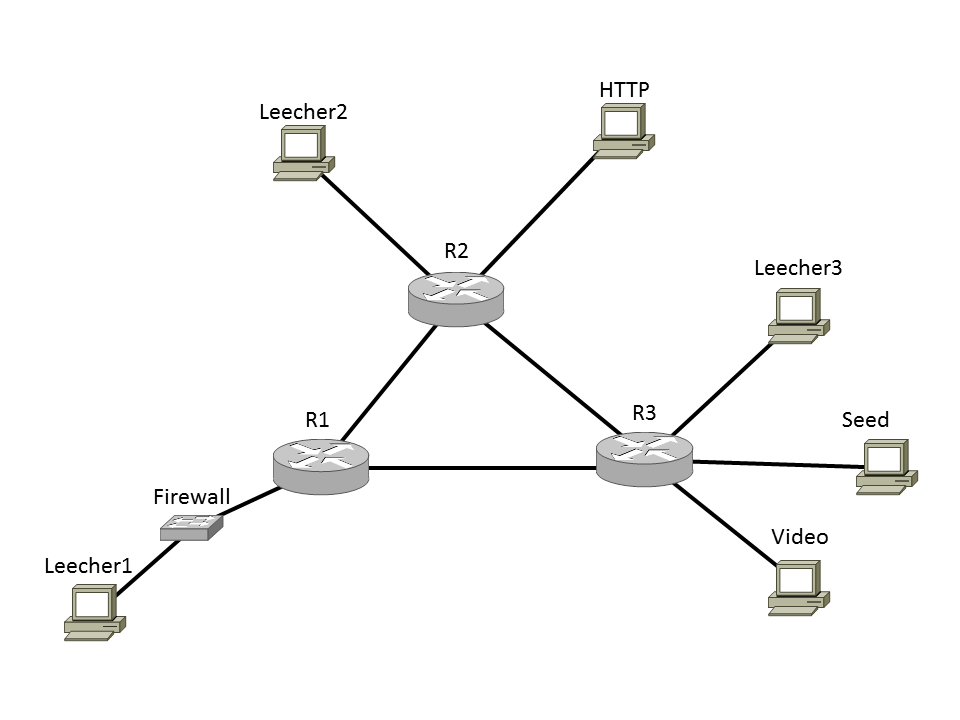
\includegraphics[width=0.9\textwidth]{figures/halozat.png}
	\caption{Network architecture used in lab exercises}
	\label{fig:Lab-topo}
\end{figure}

A hálózatban 4 OpenFlow switch fut, ezekböl 3 (R1, R2, R3) router müködést szimulál static routeokkal. Kiemelendö a szimuláció, ugyanis az OpenFlow switchek nem képesek ARP kérésekre válaszolni, így azokat vagy egy megfelelö kontroller alkalmazásból kell kezelni, vagy esetünkben static MAC címeket használunk. A szimulált hálózatban alapszabály, hogy a hostok a saját routereiket mint gatewayt mindig a csupa nullás (egyébként invalid) MAC címmel érhetik el. A hostok MAC címjei pedig "00:00:<ROUTER-ID>:00:00:<ROUTER-LINK-ID>" séma alapján kerül kiosztásra. Ennek megfelelöen az R2-es routerre kötött elsö host (leecher 2) a "00:00:02:00:00:01" MAC címmel rendelkezik.

Az R2-es routeren a következö OpenFlow statikus szabályok kerülnek beillesztésre:

\begin{lstlisting}[language=bash,frame=single,breaklines,caption={R2 router flow entry configuration},label=lst:R2-flow-config]
ovs-ofctl add-flow r2 'ip,nw_dst=89.97.0.0/16,action=mod_dl_src:00:00:00:00:00:00,output:4'
ovs-ofctl add-flow r2 'ip,nw_dst=201.42.54.65/28,action=mod_dl_src:00:00:00:00:00:00,output:5'
ovs-ofctl add-flow r2 'ip,nw_dst=23.53.32.53/32,action=mod_dl_dst:00:00:02:00:00:01,output:1'
ovs-ofctl add-flow r2 'ip,nw_dst=23.99.30.4/32,action=mod_dl_dst:00:00:02:00:00:02,output:2'
ovs-ofctl add-flow r2 'ip,nw_dst=23.0.3.78/32,action=mod_dl_dst:00:00:02:00:00:03,output:3'
ovs-ofctl add-flow r2 'arp,action=output:1,2,3' 
\end{lstlisting}

Az elsö két szabály a két szomszédos router IP cím tartományát fedi le. Látható, hogy a szomszédos routerek tartományai /16 és /28-as netmaskkal rendelkeznek. Ha ezekben az IP tartományokban érkezik egy csomag, akkor történik egy forrás MAC állítás (cél MAC állításra is szükség lenne a pontos router müködés szimulálására, de esetünkben ez kihagyható, mivel a túloldalon is általunk programozott OpenFlow eszköz van - egyszerübb flow bejegyzések) és kiküldés a megfelelö porton. Hostok esetében a match pontosan akkor törénik, ha az IP címnek mind a 32 bitje felveszi a célcímben megadott IP címet. Egyezés esetén a cél MAC a host MAC címe lesz, és kiküldi a switch/router a megfelelö porton. Az utolsó sor azt a könnyítést adja, hogy ugyanazon a subneten levö hostoknak (azaz ugyanarra a switchre/routerre bekötött) ne kelljen statikusan megadni a MAC címjeit. Mivel az ARP egy broadcast címre épülö protokoll, ezért floodolni kell, ugyanakkor figyelemben kell tartani, hogy nem minden portra kell floodolni. A router szétbontja a hálózatokat broadcast domainekre, így a router szimulációjánál is figyelembe kell venni ezt a tulajdonságot. Ha az OpenFlow switchnek flood paramétert adnánk meg, akkor a többi routert szimuláló switchnek is elküldenénk, amik szintúgy továbbítanák minden portjukon, azaz egyetlen ARP csomag képes olyan broadcast stormot generálni, ami megbénítja a Mininet szimulációt futtató gazdagépet.

A 4. switch (Firewall) nem rendelkezik statikus OF bejegyzésekkel, tisztán a kontrollertöl függ. A mérési feladatok során a kontroller programozásával kell szürésí intelligenciát vinni a tüzfalba, hogy a torrent forgalmat megfelelöen szürje, vagy éppen shape-elje. A tüzfal két porttal rendelkezik, és alapbeállításban a kontroller egy repeater funkciót valósít meg a switchen, azaz ami egyik porton beérkezik, az a másikon kimegy. A tüzfal a kontroller fele Packet-In üzenetekben küldi az egyik porton beérkezett csomagot, és ennek megfelelöen a POX kontroller alkalmazás a handlePacketIn metódusában kezeli le ezeket a csomagokat. Az intelligenciát is ebben a metódusban kell implementálni. A beérkezett csomag parsolását a következö függvényhívás végzi:
\begin{lstlisting}[language=python,frame=single,breaklines]
packet = event.parsed  
\end{lstlisting}

Ez után a 'packet' objektumtól már egyszerüen lekérdezhetöek az OpenFlow által ismert paraméterek. Például a beérkezö port sorszáma a "packet.port", míg egy specifikus TCP port megtalálása és szürése a következöképpen nézhet ki:

\begin{lstlisting}[language=python,frame=single,breaklines]
tcpp = event.parsed.find( 'tcp' )

if not tcpp: return # Not TCP

if tcpp.srcport in block_ports or tcpp.dstport in block_ports:

# Halt the event, stopping l2_learning from seeing it

# (and installing a table entry for it)

core.getLogger( "blocker" ).debug( "Blocked TCP %s <-> %s" ,

tcpp.srcport, tcpp.dstport)

event.halt = True
\end{lstlisting}

Mivel az OpenFlow nem néz L4-nél magasabb rétegekbe, ezért például egy BitTorrent csomag header mezöinek az elemzése problémásabb, ilyenkor muszáj az L4-es payload elemzése a "payload" property segítségével.

\appendix

\begin{itemize}

	\item p2pMeresTopo.py.txt: Mininet topologia P2P mereshez, futtatas: 'sudo python p2pMeresTopo.py'

	\item p2p.py.txt: POX kontroller alkalmazas, bemasolando pox/ext konyvtarba, futtatas: './pox.py p2p'
\end{itemize}

\end{document}